\documentclass[a4paper]{article}
\usepackage[utf8]{inputenc}
\usepackage[spanish, es-tabla, es-noshorthands]{babel}
\usepackage[table,xcdraw]{xcolor}
\usepackage[a4paper, footnotesep = 1cm, width=20cm, top=2.5cm, height=25cm, textwidth=18cm, textheight=25cm]{geometry}
%\geometry{showframe}

\usepackage{tikz}
\usepackage{amsmath}
\usepackage{amsfonts}
\usepackage{amssymb}
\usepackage{float}
\usepackage{graphicx}
\usepackage{caption}
\usepackage{subcaption}
\usepackage{multicol}
\usepackage{multirow}
\setlength{\doublerulesep}{\arrayrulewidth}
\usepackage{booktabs}
\usepackage{mathrsfs,amsmath}
\usepackage{hyperref}
\hypersetup{
    colorlinks=true,
    linkcolor=blue,
    filecolor=magenta,      
    urlcolor=blue,
    citecolor=blue,    
}

\newcommand{\quotes}[1]{``#1''}
\usepackage{array}
\newcolumntype{C}[1]{>{\centering\let\newline\\\arraybackslash\hspace{0pt}}m{#1}}
\usepackage[american]{circuitikz}
\usetikzlibrary{calc}
\usepackage{fancyhdr}
\usepackage{units} 

\graphicspath{./Imagenes}

\pagestyle{fancy}
\fancyhf{}
\lhead{22.05 ASSD}
\rhead{Mechoulam, Lambertucci, Rodriguez, Londero}
\rfoot{Página \thepage}

\begin{document}

%%%%%%%%%%%%%%%%%%%%%%%%%
%		Caratula		%
%%%%%%%%%%%%%%%%%%%%%%%%%

\begin{titlepage}
\newcommand{\HRule}{\rule{\linewidth}{0.5mm}}
\center
\mbox{\textsc{\LARGE \bfseries {Instituto Tecnológico de Buenos Aires}}}\\[1.5cm]
\textsc{\Large 22.05 Análisis de Señales y Sistemas Digitales}\\[0.5cm]


\HRule \\[0.6cm]
{ \Huge \bfseries Trabajo práctico N$^{\circ}$2}\\[0.4cm] 
\HRule \\[1.5cm]


{\large

\emph{Grupo 3}\\
\vspace{3px}

\begin{tabular}{lr} 	
\textsc{Mechoulam}, Alan  &  58438\\
\textsc{Lambertucci}, Guido Enrique  & 58009 \\
\textsc{Rodriguez Turco}, Martín Sebastian  & 56629 \\
\textsc{Londero Bonaparte}, Tomás Guillermo  & 58150 \\
\end{tabular}

\vspace{20px}

\emph{Profesores}\\
Jacoby, Daniel Andres\\
Belaustegui Goitia, Carlos F.\\
Iribarren, Rodrigo Iñaki\\
\vspace{3px}
%\textsc{} \\	

\vspace{100px}

\begin{tabular}{ll}

Presentado: & 15/05/20\\

\end{tabular}

}

\vfill

\end{titlepage}


%%%%%%%%%%%%%%%%%%%%%
%		Indice		%
%%%%%%%%%%%%%%%%%%%%%

\tableofcontents
\newpage

%%%%%%%%%%%%%%%%%%%%%
%		Informe		%
%%%%%%%%%%%%%%%%%%%%%

%\section{Ejercicio 1}
%	\label{Ejercicio-1}
%	\documentclass[a4paper]{article}
\usepackage[utf8]{inputenc}
\usepackage[spanish, es-tabla, es-noshorthands]{babel}
\usepackage[table,xcdraw]{xcolor}
\usepackage[a4paper, footnotesep = 1cm, width=20cm, top=2.5cm, height=25cm, textwidth=18cm, textheight=25cm]{geometry}
%\geometry{showframe}

\usepackage{tikz}
\usepackage{amsmath}
\usepackage{amsfonts}
\usepackage{amssymb}
\usepackage{float}
\usepackage{graphicx}
\usepackage{caption}
\usepackage{subcaption}
\usepackage{multicol}
\usepackage{multirow}
\setlength{\doublerulesep}{\arrayrulewidth}
\usepackage{booktabs}
\usepackage{mathrsfs,amsmath}
\usepackage{hyperref}
\hypersetup{
    colorlinks=true,
    linkcolor=blue,
    filecolor=magenta,      
    urlcolor=blue,
    citecolor=blue,    
}

\newcommand{\quotes}[1]{``#1''}
\usepackage{array}
\newcolumntype{C}[1]{>{\centering\let\newline\\\arraybackslash\hspace{0pt}}m{#1}}
\usepackage[american]{circuitikz}
\usetikzlibrary{calc}
\usepackage{fancyhdr}
\usepackage{units} 

\graphicspath{./Imagenes}

\pagestyle{fancy}
\fancyhf{}
\lhead{22.05 ASSD}
\rhead{Mechoulam, Lambertucci, Rodriguez, Londero}
\rfoot{Página \thepage}

\begin{document}

\subsection{Introducción}

\subsection{Conversor ADC0808}

El ADC0808 es un conversor analógico-digital de ocho bits con ocho canales multiplexados y salida binaria paralela. En el presente informe se utilizó un único canal analógico. Este conversor está compuesto por una red en escalera 256R conectada a un árbol de llaves, el cual compara los distintos valores proporcionados por la red 256R con la entrada analógica. Es así —mediante el registro de aproximaciones sucesivas, el cual realiza una búsqueda binaria con todos los valores posibles de la red escalera hasta converger a un valor digital óptimo— que logra el ADC0808 realizar la conversión analógica-digital.

\begin{figure}[H]
\centering
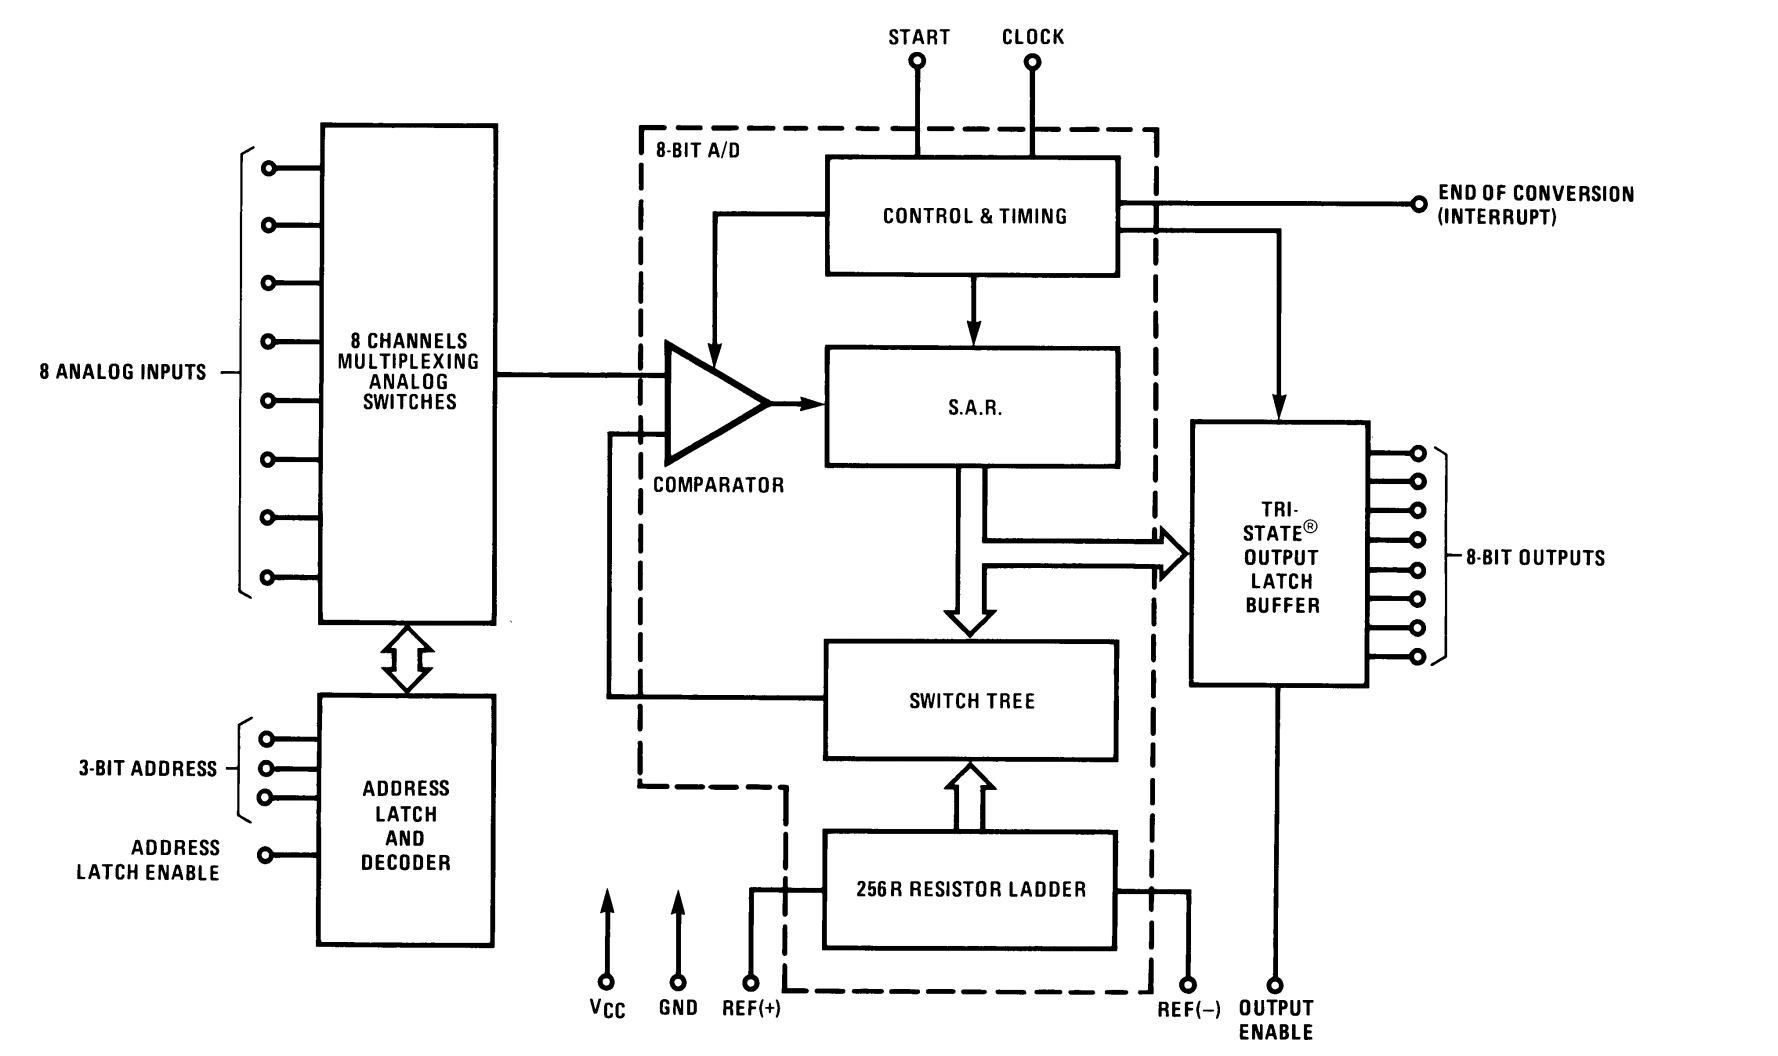
\includegraphics[width=0.75\linewidth]{ImagenesEjercicio1/ADC_BLOCK.png}
\caption{Diagrama en bloques simplificado del conversor ADC0808.}
\label{ADC_BLOCK}
\end{figure}

A continuación, se detallará la funcionalidad de cada pin del integrado mostrado en la Figura (\ref{ADC_BLOCK}) de manera simplificada donde se puede observar el diagrama temporal en la Figura (\ref{ADC_TIMING}).

\begin{itemize}
\item \textbf{8 Analog Inputs}: Aquí se colocan las entradas analógicas que se desean convertir. Se utilizó únicamente una sola de estas entradas, mientras que el resto se las conectó a tierra para evitar el ruido electromagnético.
\item \textbf{3-bit Adress}: Esta entrada binaria permite seleccionar qué entrada analógica se utilizará para realizar la conversión. Estas entradas se conectaron permanentemente a tierra, de manera tal que siempre se realice la conversión con la primer entrada analógica.
\item \textbf{Adress Latch Enable}: Para un valor alto, el ADC0808 mantendrá registro del último adress ingresado. Se conectó a VCC.
\item \textbf{VCC}: Tensión positiva de alimentación, se utilizó el valor de $5.12V$ de tal manera que la resolución a la salida sea de $20mV$ por bit.
\item \textbf{GND}: Tierra del circuito
\item \textbf{REF(+), REF(-)}: Tensiones de referencia para la red escalera 256R. Se conectó la referencia positiva a VCC y la negativa a GND.
\item \textbf{Clock}: El clock utilizado fue el típico extraído de la datasheet, de $640kHz$.
\item \textbf{Start}: Esta señal de control inicia un ciclo de conversión.
\item \textbf{End of Conversion}: Esta señal de interrupción pasa a un estado alto cuando se acaba un ciclo de conversión. Si se conecta esta señal a la señal de \textbf{Start} se logra la máxima frecuencia de conversión para una señal de \textbf{Clock} fija.
\item \textbf{8-bit Outputs}: Salida digital paralela de ocho bits.
\item \textbf{Output Enable}: Permite utilizar la funcionalidad tri-state del buffer de salida. Este pin no fue utilizado.
\end{itemize}

\begin{figure}[H]
\centering
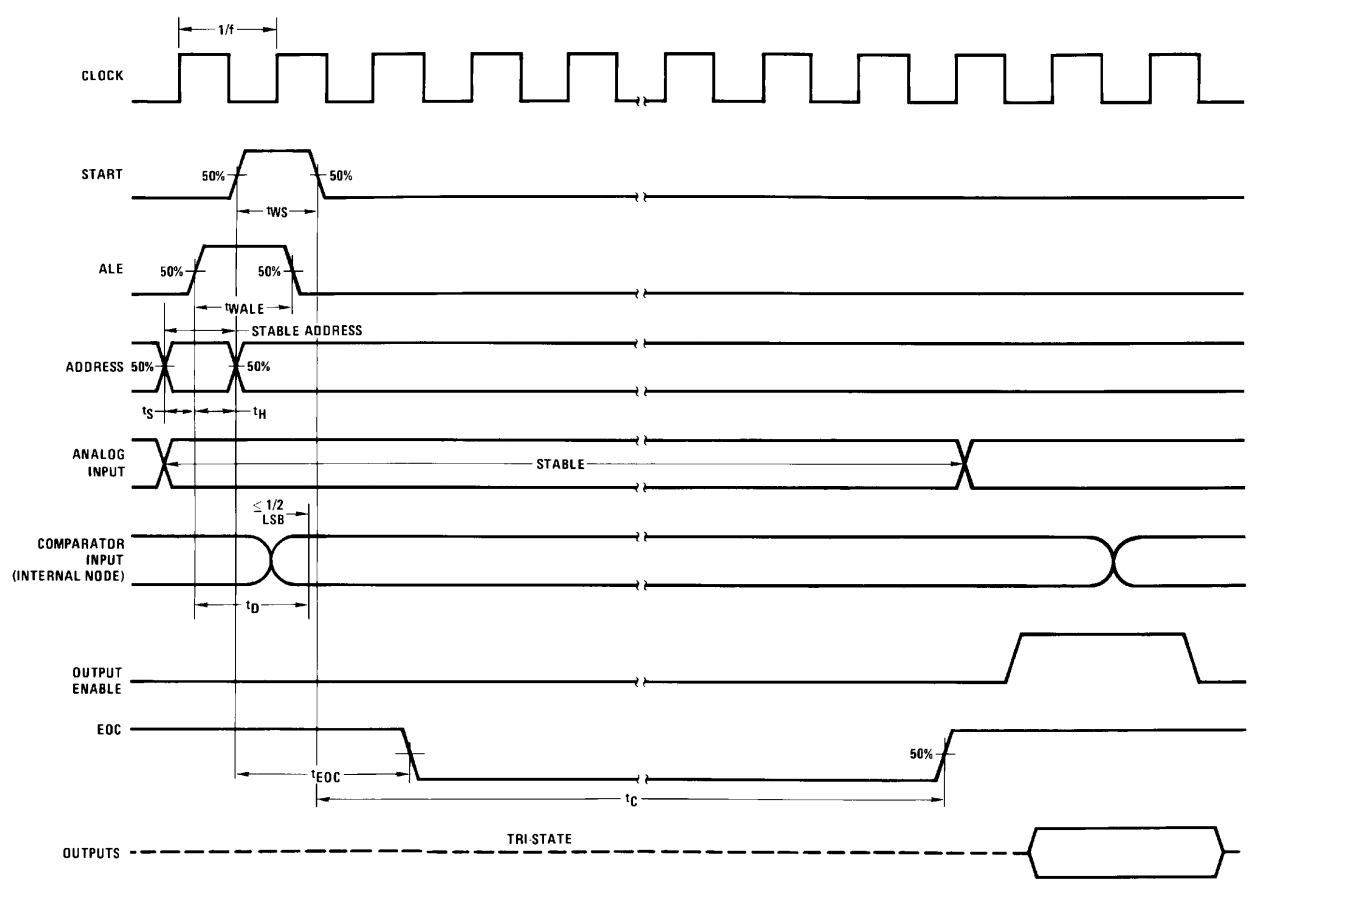
\includegraphics[width=0.9\linewidth]{ImagenesEjercicio1/ADC_TIMING.png}
\caption{Diagrama temporal de las señales de entrada, salida y control del conversor ADC0808.}
\label{ADC_TIMING}
\end{figure}

\subsection{Acondicionamiento de la señal de entrada}

\subsubsection{Offset y enclavamiento}

Dado que la señal que ingresa al ADC0808 debe estar contenida dentro del rango $0V$—$5.12V$ con un margen de $100mV$, se montó a la señal de entrada sobre un nivel de continua igual a $\frac{5.12V - 0V}{2} = 2.56V$ para luego limitar con un circuito enclavador a esta resultante entre los rangos permisibles del conversor. El circuito utilizado se detalla en la Figura (\ref{ACOND}).

\begin{figure}[H]
\centering
\includegraphics[width=0.8\linewidth]{ImagenesEjercicio1/ada.pdf}
\caption{Circuito de acondicionamiento de la señal de entrada.}
\label{ACOND}
\end{figure}

\subsubsection{Sample and Hold}

A la hora de realizar el proceso de conversión, el comparador del ADC necesita que la señal de entrada se mantenga estable. Como se vio en la sección anterior, si no se utiliza un sample & hold, es necesario que la frecuencia de entrada sea lo suficientemente baja como para que el comparador logre hacer su trabajo sin comprometer la precisión de este.

El S \& H seleccionado es el \href{https://pdf1.alldatasheet.es/datasheet-pdf/view/8580/NSC/LF398N.html}{LF398N}. Sabiendo que se posee una taza de conversión máxima de $8.62 \ kHz$, impuesta por el tiempo máximo de conversión del ADC0808 de $116 \mu s$, lo que implica que

\begin{equation*}
	T_{acq} = \frac{2}{8.62 \ kHz} \approx 232 \mu s
\end{equation*}

De esta forma, observando el gráfico de la hoja de datos mostrada en la Figura (\ref{chacqtime}) del S\& H, se requiere un capacitor de $80 \ nF$.

\begin{figure}[H]
	\centering
	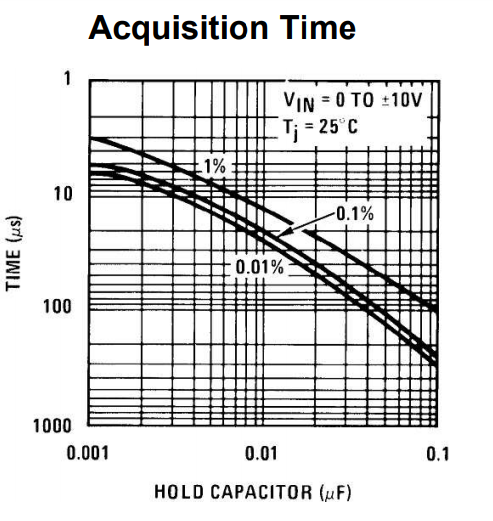
\includegraphics[width=0.3\textwidth]{ImagenesEjercicio1/chacqtime.png}
\caption{Tiempo de adquisición del S \& H en función del capacitor de hold.}
	\label{chacqtime}
\end{figure}

\subsection{Máxima frecuencia de entrada sin Sample \& Hold}

De la datasheet del ADC0808, se tiene que si $V_{CC} = V_{REF+} = 5.12V$ y $V_{REF-} = 0V$, la resolución será de $20 \frac{mV}{bit}$. Si se utiliza la frecuencia de clock $f_{CLK}$ típica utilizada en la datasheet de $640kHz$, el tiempo de conversión $t_C$ máximo será de $116\mu s$. Esto implica que la entrada no deberá de tener una pendiente mayor a $\frac{20mV}{116\mu s}$ para no introducir error en la cuantización de la señal.


Si la señal de entrada se encuentra en el peor caso, es decir, con una excursión de tensión de $-0.1V + V_{REF-}$ a $5.12V + 0.1V$; esta se encuentra montada sobre un nivel de continua igual a $(5.22V - (-0.1V))/2 = 2.66V$; y esta se puede considerar senoidal gracias a la teoría desarrollada por Fourier; se tiene que la amplitud pico máxima de la senoidal podrá ser $2.66V$. Luego, asumiendo el peor caso de la pendiente de la senoidal, para un ángulo igual a cero radianes, lo que permite utilizar la aproximación paraxial, se tiene que
\\

\begin{equation}
\left. \frac{d \left( 2.66V \cdot Sin \left( 2\pi f_{in_{max}} t \right) \right)}{dt} \right|_{t=0} = 2.66V \cdot 2\pi f_{in_{max}} = \frac{20mV}{116\mu s}
\end{equation}
\\


Finalmente, se obtiene que la componente de mayor frecuencia de la señal de entrada para no comprometer la precisión del ACD0808 deberá ser como máximo

$$f_{in_{max}} = 10.3Hz$$

\subsection{Conversor DAC0800}
Se utilizó el integrad DAC0800, un conversor D/A de 8 bits con salida diferencial de corriente.
Para convertir esta corriente en un nivel de tensión se utilizó el circuito propuesto por la hoja de datos que se muestra a continuación:
\begin{figure}[H]
	\centering
	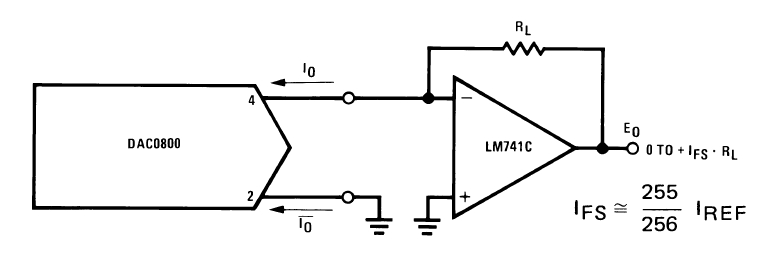
\includegraphics[width=0.8\textwidth]{ImagenesEjercicio1/dacout.png}
\caption{Configuración saldia DAC.}
	\label{fig:dacout}
\end{figure}
La salida va de 0 a $V_{fs}= I_{fs}cdot R_L$.\\
En cuanto al pinout del DAC es el siguiente:
\begin{figure}[H]
	\centering
	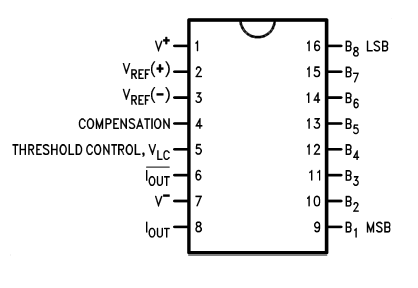
\includegraphics[width=0.5\textwidth]{ImagenesEjercicio1/dacpinout.png}
\caption{Pinout DAC0800.}
	\label{fig:dapinout}
\end{figure}
Donde los pines desde B1 a B8 son las entradas digitales, siendo B1 el bit mas significativo. En cuanto a la salida, es por corriente, y corresponde a los pines 6 y 8, cabe mencionar que dichas corrientes son complementaria, osea su suma da 0. Los pines 2 y 3 son las tensiones $V^+$ Y $V^-$ fueron conectadas a 5V y a GND respectivamente, mientras que las tensiones de referencia, si bien dice tensiones, uno debe proveer corrientes de referencia, esto se hace utilizando una resistencia entre vcc y $V_{ref^+}$, al igual que una entre GND y $V_{ref^-}$. En cuanto al pin de threshold fue conectado a masa, finalmente en el pin de comp se conectó un capacitor de 100nF.

\subsection{Señal de sincronización de conversión}

\subsubsection{Restricciones temporales}

Si los componentes utilizados tuviesen un tiempo de operación ideal, se podría utilizar un clock tan rápido como se quiera. Sin embargo, esto no sucede. Por parte del integrado ADC0808, se tiene que el tiempo de conversión con una señal de sincronización de $640kHz$ es como máximo $116\mu s$. Luego, el DAC0800 posee un tiempo de estabilización de $100ns$. Por parte del sample \& hold utilizado, el LF398N, se tiene que el tiempo de adquisición máximo con un capacitor de hold de $80 nF$ es de $20\mu s$. Finalmente, se obtienen dos limitantes en tiempo: 

\begin{itemize}
\item El ADC0808 tardará como máximo $116\mu s$ en convertir el valor holdeado de la señal analógica en digital.
\item El LF398N tardará como máximo $20\mu s$ en cargar el capacitor de hold con el valor de la señal analógica en la fase de sampleo.
\end{itemize}

Es por esto, que la rapidez máxima del clock que gobierna la frecuencia de conversión del circuito será el doble del mínimo entre la inversa de los dos limitantes temporales, es decir, $\frac{1}{2\cdot 116\mu s} = 4.31kHz$. Sin embargo, si que quisiese aumentar aún más las frecuencia de conversión del circuito, se podría implementar un clock cuyo duty cycle no sea del $50\%$, debido a que mientras el ADC se encuentra convirtiendo, el s\&h no posee ninguna restricción temporal más que la de fuga, mientras que si el s\&h está sampleando la señal, el ADC no posee ninguna restricción temporal.

%aca poner grafico de un clock con duty cycle no simetrico donde en la parte que dura poco se esta haciendo el sampleo y en la parte larga se esta haciendo la conversión

Basta con que el duty cycle sea tal que el tiempo de holdeo sea igual al tiempo de conversión del ADC y el tiempo de sampleo se igual al tiempo máximo que tarda el s\&h en cargar su capacitor de hold. Se tiene entonces que

\begin{equation}
DT_{optimo} = \frac{20\mu s}{116\mu s}\cdot 100 = 17.24\% 
\end{equation}

para simplificar el circuito, se tomó $DT = 25\%$ y la frecuencia de esta señal de sincronización deberá ser como máximo $\frac{1}{116\mu s + 20\mu s} = 7.352kHz$.

\subsubsection{Circuito generador de la señal de sincronización}

Se partió de un generador de onda cuadrada de $640kHz$, el cual será la señal de clock del ADC0808. Esta señal pasará además por un divisor de frecuencia que divide por $88$ veces para obtener una frecuencia menor pero cercana a $7.352kHz$, de $7.272kHz$. Luego, esta señal ingresa a dos divisores de frecuencia en cascada que dividen por dos. Se detalla en la Figura (\ref{DT}) esta operación. Luego, se realiza la operación AND entre la señal antes de pasar por los divisores en frecuencia, y las señales a la salida de cada divisor. Así se obtiene una señal de $DT$ del $25\%$ independientemente de la frecuencia de la señal original.

%aca poner grafico de guido

Esta señal posterior a la operación AND es la que se utilizará como señal de control del S\&H. Finalmente, se quiere enviar un pulso de una duración de al menos $t_{ws} = 200ns$ al pin de start del ADC0808 cuando el S\&H comience a holdear, por lo que se utilizará un negador seguido de un detector de flancos para generar esta señal de start. El resultado se detalla en la Figura (\ref{START})

\begin{figure}[H]
\centering
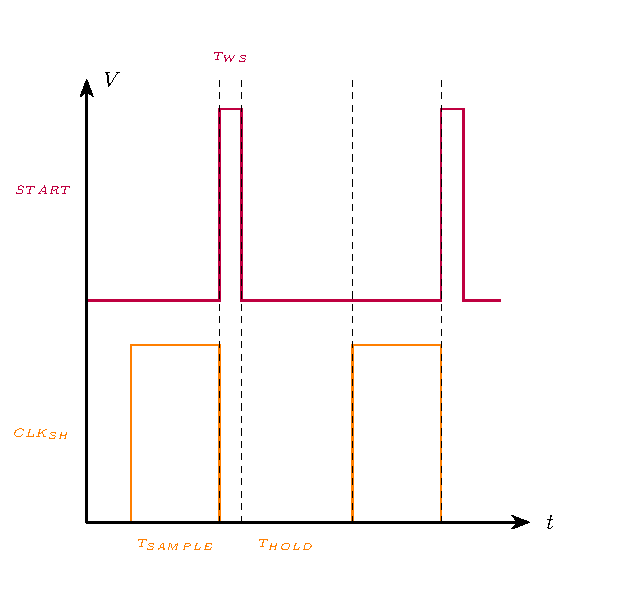
\includegraphics[width=0.8\linewidth]{ImagenesEjercicio1/Graficos.pdf}
\caption{Diagrama temporal de las señales de control del circuito.}
\label{START}
\end{figure}

Así se obtienen todas las señales de control del circuito de una misma señal de clock original, de tal manera que todas estén sincronizadas entre sí. Si se desea disminuir la frecuencia de conversión basta con disminuir la frecuencia 

\subsubsection{Circuito oscilador}

Se utilizó el circuito mostrado en la Figura (\ref{555}) para generar la señal de clock de $640kHz$ la cual no solo será ingresada al ADC0808 sino de la cual se generarán las señales de sincronización del S\&H y de start del conversor.

\begin{figure}[H]
\centering
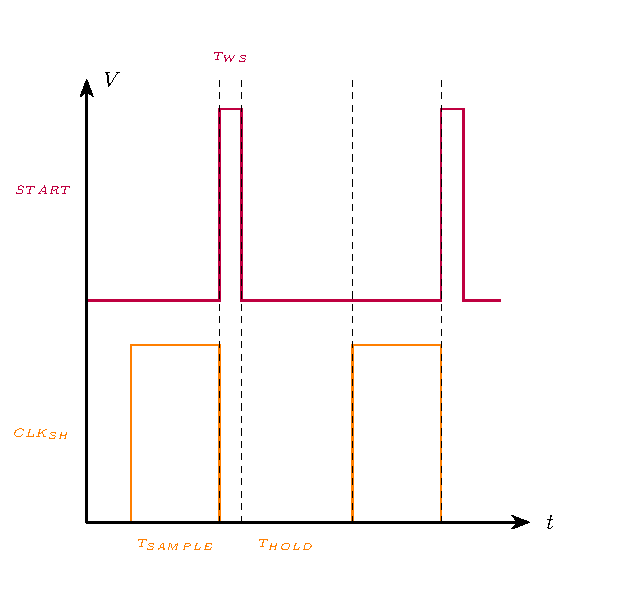
\includegraphics[width=0.8\linewidth]{ImagenesEjercicio1/Graficos.pdf}
\caption{Circuito oscilador.}
\label{START}
\end{figure}

Utilizando $R_{T} = 620 + 110\Omega$, $R_{POT} = 1k\Omega$ y $C_{T} = 1nF$ se logra obtener

\[ 49kHz < f_CLK < 632kHz\]

por lo que la frecuencia de conversión del circuito total será de

\[ 557Hz < f_CONV < 7.2kHz \]

\end{document}
%		
%\section{Ejercicio 2}
%	\label{Ejercicio-2}
%	
\subsection{Introducción}


<<<<<<< HEAD
\subsubsection{Introducción}
El conversor sigma-delta o delta-sigma según la literatura consultada, tuvo su aparición durante los años 60's y 70's. Aunque su nombre pueda sugerir un tipo de tecnología muy compleja la realidad es que no lo es en términos constructivos. Los moduladores sigma-delta nos permiten alcanzar una digitalización de alta resolución (16bits o 24bits) sin la necesidad de utilizar ADC de ese porte. Esto se consigue dado que este diseño permite alcanzar un nivel de ruido de cuantización equivalente a la de un ADC de mayor porte utilizando un ADC más modesto.
El modulador sigma-delta se vale de los beneficios del oversampling para conseguir un diseño sencillo y eficaz.
Un componente que esta presente en todos los ADC es el FAA, filtro anti-alias, que se coloca a la entrada del ADC para evitar solapamientos espectrales cuando se realiza el muestreo interno. En el caso del sigma-delta,  la señal es sobre muestreada por más de 64 por sobre la frecuencia de nyquist. Esto implica que las replicas del espectro de banda base se encontraran más alejada entre sí en el espectro.
\begin{figure}[H]
	\centering
	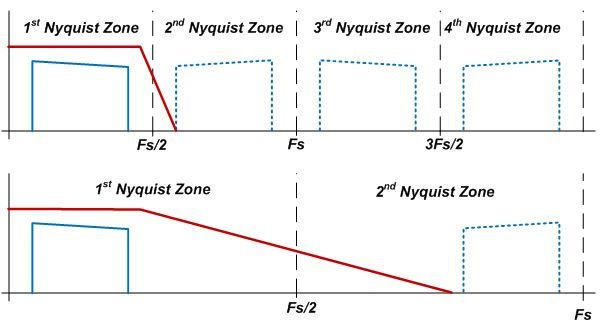
\includegraphics[width=0.7\linewidth]{ImagenesEjercicio2/Oversampling}
	\caption{Efectos del oversampling sobre las replicas espectrales}
	\label{fig:oversampling}
\end{figure}
Esto nos permite utilizar un filtro anti-alias de bajo orden, los cuales son más sencillos de realizar.


Además como se vera en secciones posteriores, el sobre-muestreo mejorara notablemente la performance de nuestro sencillo ADC de un 1-bit.

\subsubsection{Arquitectura}
=======
\subsection{Arquitectura}
>>>>>>> 67435597220b151a8b5cda66c526e8121bdc0398

A continuación presentamos la topología implementada:

\begin{figure}[H]
	\centering
	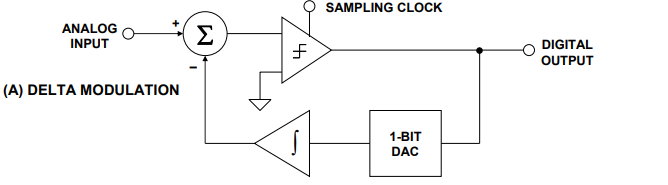
\includegraphics[width=0.7\linewidth]{ImagenesEjercicio2/diagramaEnBloques}
	\caption{Modulador $\Sigma\Delta$ de primer orden}
	\label{fig:diagramaenbloques}
\end{figure}

Como se puede observar el modulador $\Sigma\Delta$ se basa en un circuito con un solo camino de realimentación negativa que incorpora un cuantificador y un DAC en su interior.

El input analógico ingresa al sistema y se determina si el valor de la señal en ese instante es mayor o menor que su valor anterior. De esta forma conseguimos traducir la información analogica a un código binario que representa la señal en términos de los cambios en la señal.



<<<<<<< HEAD
\subsubsection{Modulador}
La salida del modulador $\Sigma\Delta$ es un bit-stream de valores binarios unipolares o bipolares, acorde al diseño utilizado. En esta secuencia se encuentra codificada toda la información necesaria para poder reconstruir la señal original. Aún más importante que reconstruir la señal original, es conseguir un valor preciso de la misma en un instante de tiempo. Es decir, poder tomar mediciones. Este tipo de conversores son famosos por la alta resolución que son capaces de proveer. Sin embargo, el limite de su funcionalidad aparece cuando se los quiere utilizar en un ambiente donde la señales cambian de forma abrupta.
=======
\subsection{Modulador}
La salida del modulador $\Sigma\Delta$ es un bit-stream de valores binario arbitrarios. En esta secuencia se encuentra codificada toda la información necesaria para poder reconstruir la señal original. Aún más importante que reconstruir la señal original, es conseguir un valor preciso de la misma en un instante de tiempo. Es decir, poder tomar mediciones. Este tipo de conversores son famosos por la alta resolución que son capaces de proveer. Sin embargo, el limite de su funcionalidad aparece cuando se los quiere utilizar en un ambiente donde la señales cambian de forma abrupta.
>>>>>>> 67435597220b151a8b5cda66c526e8121bdc0398

\begin{figure}[H]
	\centering
	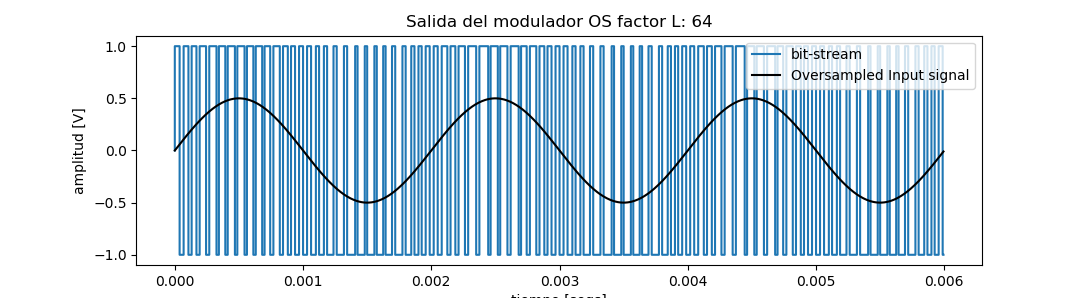
\includegraphics[width=0.7\linewidth]{ImagenesEjercicio2/BitsStream64}
	\caption{}
	\label{fig:bitsstream64}
\end{figure}


\subsection{Noise Shaping}
Una de las más notables características de este tipo de modulación es el efecto llamado \textbf{noise-shaping}. Este efecto provoca que el ruido de cuantización sea "moldeado" hacia las altas frecuencias empujándolo lejos de la banda de interés.


\begin{figure}[H]
	\centering
	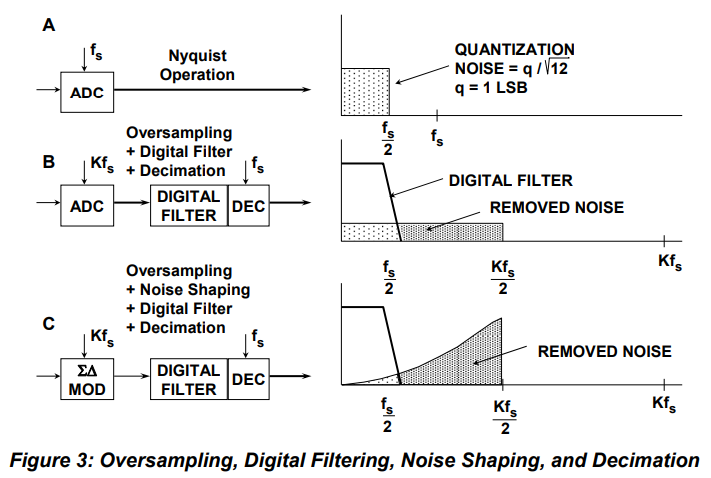
\includegraphics[width=0.7\linewidth]{ImagenesEjercicio2/NoiseShappingAN}
	\caption{}
	\label{fig:noiseshappingan}
\end{figure}


Esto implica que el ruido de cuantización efectivo, dentro de la banda de interés, se ve reducido. Esto es equivalente a pensar que la señal fue cuantizada mediante un cuantizador que tiene un ruido de cuantización proporcional al ruido restante sobre la banda de interés.

En la siguiente imagen vemos la salida del modulador, podemos elegir entre salida unipolar o monopolar dependiendo de como se realice el post-procesamiento que se le de luego de la modulación.
 
\begin{figure}[H]
	\centering
	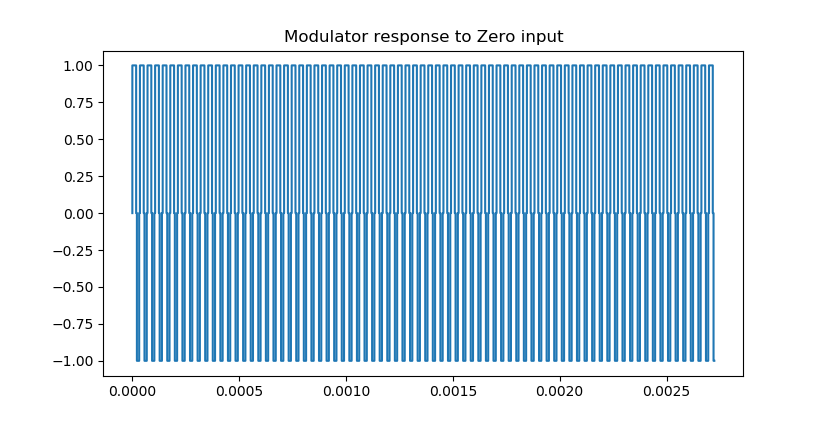
\includegraphics[width=0.7\linewidth]{ImagenesEjercicio2/OutoutZeroInput}
	\caption{Salida del modulador con Input nulo}
	\label{fig:outoutzeroinput}
\end{figure}

Podemos observar como al usar un gran frecuencia de sampleo obtenemos la caracteristica curva de noise-shaping del ruido de cuantización.
\begin{figure}[H]
	\centering
	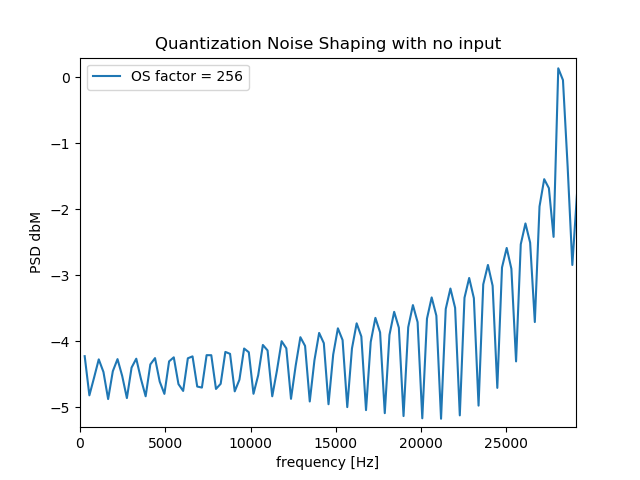
\includegraphics[width=0.7\linewidth]{ImagenesEjercicio2/QnoiseNoInput}
	\caption{}
	\label{fig:qnoisenoinput}
\end{figure}


A continuación aplicamos la modulación sigma-delta sobre una señal senoidal con una frecuencia fundamental de $500Hz$. 
\begin{figure}[H]
	\centering
	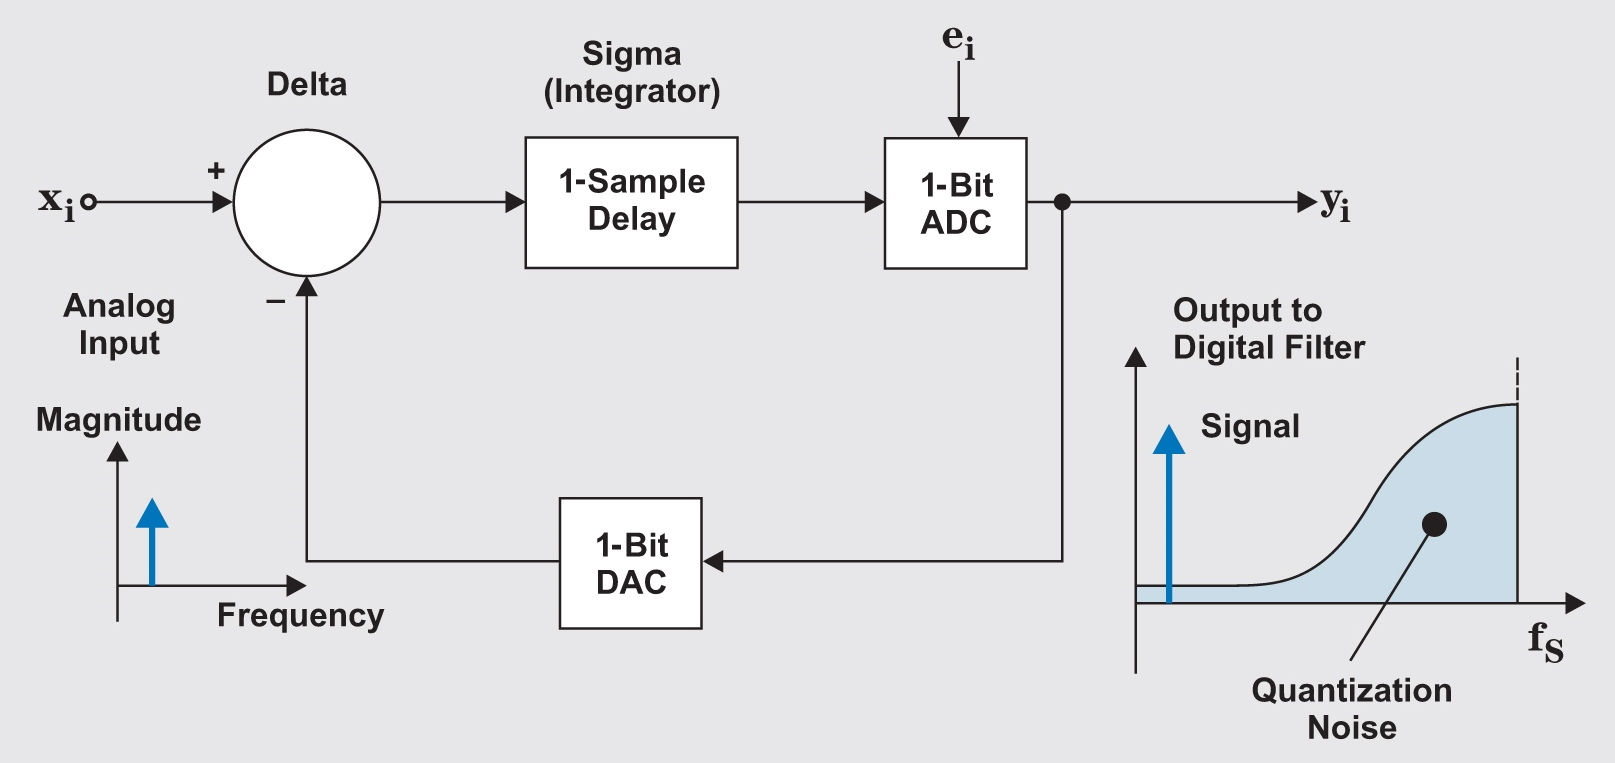
\includegraphics[width=0.7\linewidth]{ImagenesEjercicio2/NoiseShapingFullsche}
	\caption{}
	\label{fig:noiseshapingfullsche}
\end{figure}



Debajo muestran los resultados obtenidos luego de realizar el periodograma sobre los bits de salida

\begin{figure}[H]
	\centering
	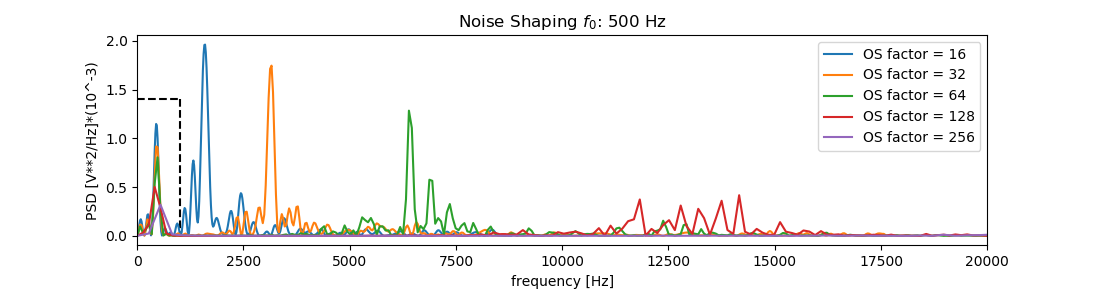
\includegraphics[width=\linewidth]{ImagenesEjercicio2/NoiseShappingDemo1zoom2solid.png}
	\caption{Noise Shapping con diferentes niveles de sobremuestreo}
	\label{fig:noiseshappingdemo1}
\end{figure}
En primer lugar podemos ver que a medida que aumentamos la tasa de oversampling (OS), el ruido de cuantización se aleja más de la banda de interés e incursiona hacia posiciones más elevadas en el espectro.

\begin{figure}[H]
	\centering
	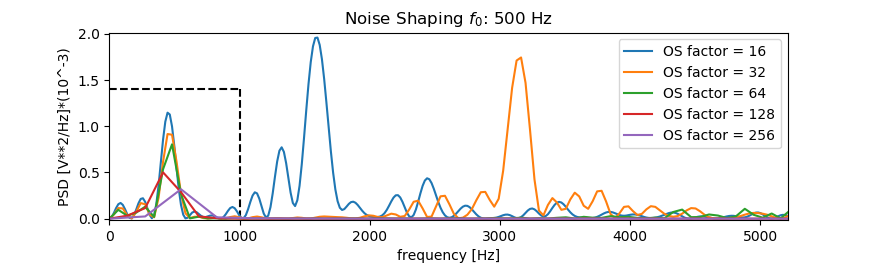
\includegraphics[width=\linewidth]{ImagenesEjercicio2/NoiseShappingSolidZoom.png}
	\caption{Noise Shapping con diferentes niveles de sobremuestreo, acercamiento}
	\label{fig:noiseshappingdemo1}
\end{figure}

Si reescalamos la potencia espectral y la expresamos en dBm conseguimos apreciar notoriamente el noise-shapping.

El pico observado a bajas frecuencias corresponde a la frecuencia fundamental de nuestra información de entrada
\begin{figure}[H]
	\centering
	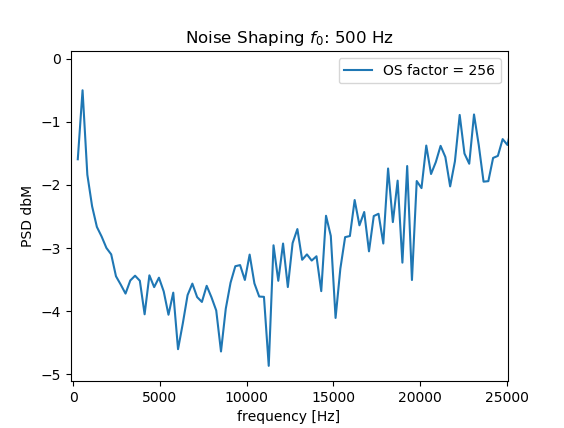
\includegraphics[scale=0.7]{ImagenesEjercicio2/NoiseShappingdbM.png}
	\caption{Noise Shapping}
	\label{fig:noiseshappingdemo1}
\end{figure}
<<<<<<< HEAD

\subsubsection{Decimación}
El objetivo de sobremuestrear la señal era el de aumentar la resolución de nuestro ADC. Sin embargo, la tasa de información generada puede ser demasiado alta como para que la circuiteria posterior pueda manejarla de manera efectiva. Es por eso que luego del proceso de modulación se filtra la señal de salida y se reduce la cantidad de muestras de la misma.

Debajo se pueden ver diversos experimentos realizados.

\begin{figure}[H]
	\centering
	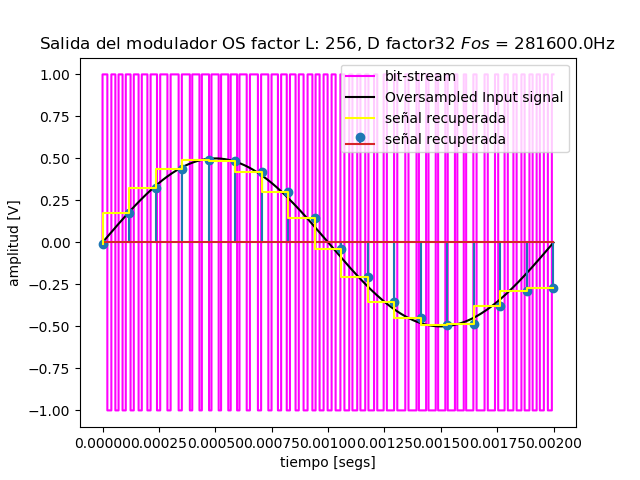
\includegraphics[width=0.7\linewidth]{ImagenesEjercicio2/SenalRecuperada256.png}
	\caption{}
	\label{fig:senalrecuperada256}
\end{figure}
\begin{figure}[H]
	\centering
	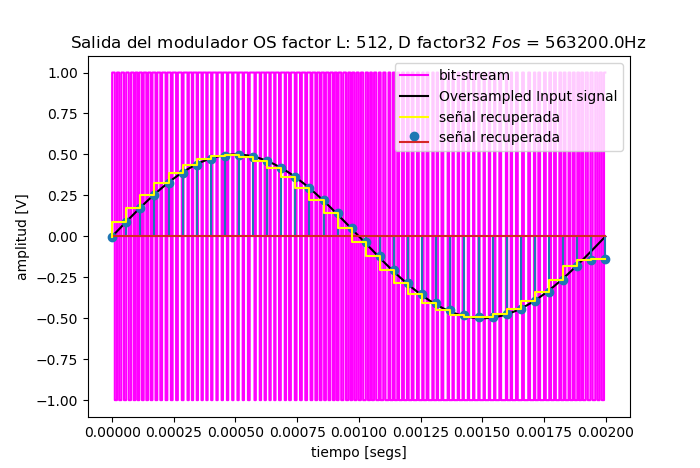
\includegraphics[width=0.7\linewidth]{ImagenesEjercicio2/SenalRecuperada512.png}
	\caption{}
	\label{fig:senalrecuperada256}
\end{figure}

\subsubsection{Simulaciones}
Se realizaron las simulaciones íntegramente en Python, se recomienda correr el archivo \textbf{demos.py} para ver todas las demostraciones.

\end{document}
=======
>>>>>>> 67435597220b151a8b5cda66c526e8121bdc0398

%	
\section{Síntesis de sonidos mediante frecuencia modulada}
	\label{Ejercicio-3}
	\documentclass[a4paper]{article}
\usepackage[utf8]{inputenc}
\usepackage[spanish, es-tabla, es-noshorthands]{babel}
\usepackage[table,xcdraw]{xcolor}
\usepackage[a4paper, footnotesep = 1cm, width=20cm, top=2.5cm, height=25cm, textwidth=18cm, textheight=25cm]{geometry}
%\geometry{showframe}

\usepackage{tikz}
\usepackage{amsmath}
\usepackage{amsfonts}
\usepackage{amssymb}
\usepackage{float}
\usepackage{graphicx}
\usepackage{caption}
\usepackage{subcaption}
\usepackage{multicol}
\usepackage{multirow}
\setlength{\doublerulesep}{\arrayrulewidth}
\usepackage{booktabs}
\usepackage{mathrsfs,amsmath}
\usepackage{hyperref}
\hypersetup{
    colorlinks=true,
    linkcolor=blue,
    filecolor=magenta,      
    urlcolor=blue,
    citecolor=blue,    
}

\newcommand{\quotes}[1]{``#1''}
\usepackage{array}
\newcolumntype{C}[1]{>{\centering\let\newline\\\arraybackslash\hspace{0pt}}m{#1}}
\usepackage[american]{circuitikz}
\usetikzlibrary{calc}
\usepackage{fancyhdr}
\usepackage{units} 

\graphicspath{./Imagenes}

\pagestyle{fancy}
\fancyhf{}
\lhead{22.05 ASSD}
\rhead{Mechoulam, Lambertucci, Rodriguez, Londero}
\rfoot{Página \thepage}

\begin{document}

Las llaves compuestas por tecnología de estado solido son pequeñas, rápidas, de fácil uso y control. Además poseen un consumo bajo comparado con compuertas tradicionales controladas electricamente.

Las compuertas digitales estan diseñadas para que transmitir y bloquear señales de niveles digitales. Por otro lado, las analógicas son diseñados para señales analógicas, si bien normalmente presentan un buen comportamiento frente a las digitales.

\subsection{\href{http://www.ti.com/lit/ds/symlink/cd4016b.pdf}{CD4016}}
\begin{multicols}{2}
\begin{itemize}
	\item $V_{OS} = 0.4 \ V \sim 13.5 \ V$
	\item Resistencia ``on-state'' $= 400 \ \Omega \sim 2 \ k\Omega$
	\item $TDH = 0.4\%$
	\item Capacidad de entrada $C_{is} = 4 \ pF$
	\item Capacidad de salida $C_{os} = 4 \ pF$
	\item Capacidad Feedthrough $C_{ios} = 0.2 \ pF$
	\item Crosstalk $= 50 \ mV$
	\item Delay de encendido/apagado $= 15 \ ns \sim 70 \ ns$
\end{itemize}
\end{multicols}

\subsection{\href{http://www.ti.com/lit/ds/symlink/cd4066b.pdf}{CD4066}, \href{http://www.ti.com/lit/ds/symlink/cd4051b.pdf}{CD4053} y \href{http://www.ti.com/lit/ds/symlink/cd4051b.pdf}{CD4051}}
\begin{multicols}{2}
\begin{itemize}
	\item $V_{OS} = 0.4 \ V \sim 13.5 \ V$
	\item Resistencia ``on-state'' $= 200 \ \Omega \sim 1.3 \ k\Omega$
	\item $TDH = 0.4\%$
	\item Capacidad de entrada $C_{is} = 8 \ pF$
	\item Capacidad de salida $C_{os} = 8 \ pF$
	\item Capacidad Feedthrough $C_{ios} = 0.5 \ pF$
	\item Crosstalk $= 50 \ mV$
	\item Delay de encendido/apagado $= 15 \ ns \sim 70 \ ns$
\end{itemize}
\end{multicols}
Estos datos varían dependiendo en $VDD$, entre $5 \ V$ y $15 \ V$.


\end{document}

\section{Introducción modelo Karplus-Strong}
	\label{Ejercicio-4}
	\documentclass[a4paper]{article}
\usepackage[utf8]{inputenc}
\usepackage[spanish, es-tabla, es-noshorthands]{babel}
\usepackage[table,xcdraw]{xcolor}
\usepackage[a4paper, footnotesep = 1cm, width=20cm, top=2.5cm, height=25cm, textwidth=18cm, textheight=25cm]{geometry}
%\geometry{showframe}

\usepackage{tikz}
\usepackage{amsmath}
\usepackage{amsfonts}
\usepackage{amssymb}
\usepackage{float}
\usepackage{graphicx}
\usepackage{caption}
\usepackage{subcaption}
\usepackage{multicol}
\usepackage{multirow}
\setlength{\doublerulesep}{\arrayrulewidth}
\usepackage{booktabs}
\usepackage{mathrsfs,amsmath}
\usepackage{hyperref}
\hypersetup{
    colorlinks=true,
    linkcolor=blue,
    filecolor=magenta,      
    urlcolor=blue,
    citecolor=blue,    
}

\newcommand{\quotes}[1]{``#1''}
\usepackage{array}
\newcolumntype{C}[1]{>{\centering\let\newline\\\arraybackslash\hspace{0pt}}m{#1}}
\usepackage[american]{circuitikz}
\usetikzlibrary{calc}
\usepackage{fancyhdr}
\usepackage{units} 

\graphicspath{./Imagenes}

\pagestyle{fancy}
\fancyhf{}
\lhead{22.05 ASSD}
\rhead{Mechoulam, Lambertucci, Rodriguez, Londero}
\rfoot{Página \thepage}

\begin{document}

\subsection{Introducción modelo Karplus-Strong}
En esta sección se analizará el método de sintesis basado en el modelado físico, propuesto por Karplus-Strong.
\subsection{Karplus-Strong básico}
El modelo básico de Karplus-Strong consiste filtrar una forma de onda a travez de una linea de retardo, gracias a esto se logra simular el sonido de una cuerda de guitarra.
\begin{figure}[H]
	\centering
	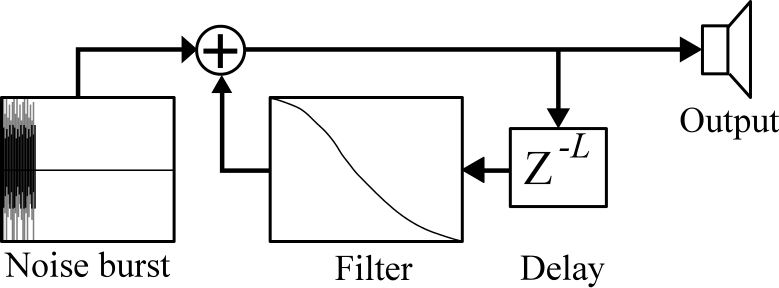
\includegraphics[width=0.8\textwidth]{ImagenesEjercicio4/ksinit.PNG}
\caption{Modelo clásico Karplus-Strong.}
	\label{fig:kscl}
\end{figure}
\subsubsection{Análisis teórico}
Este algoritmo se puede describir por su diagrama en bloques como se ve  a continuación.
\begin{figure}[H]
	\centering
	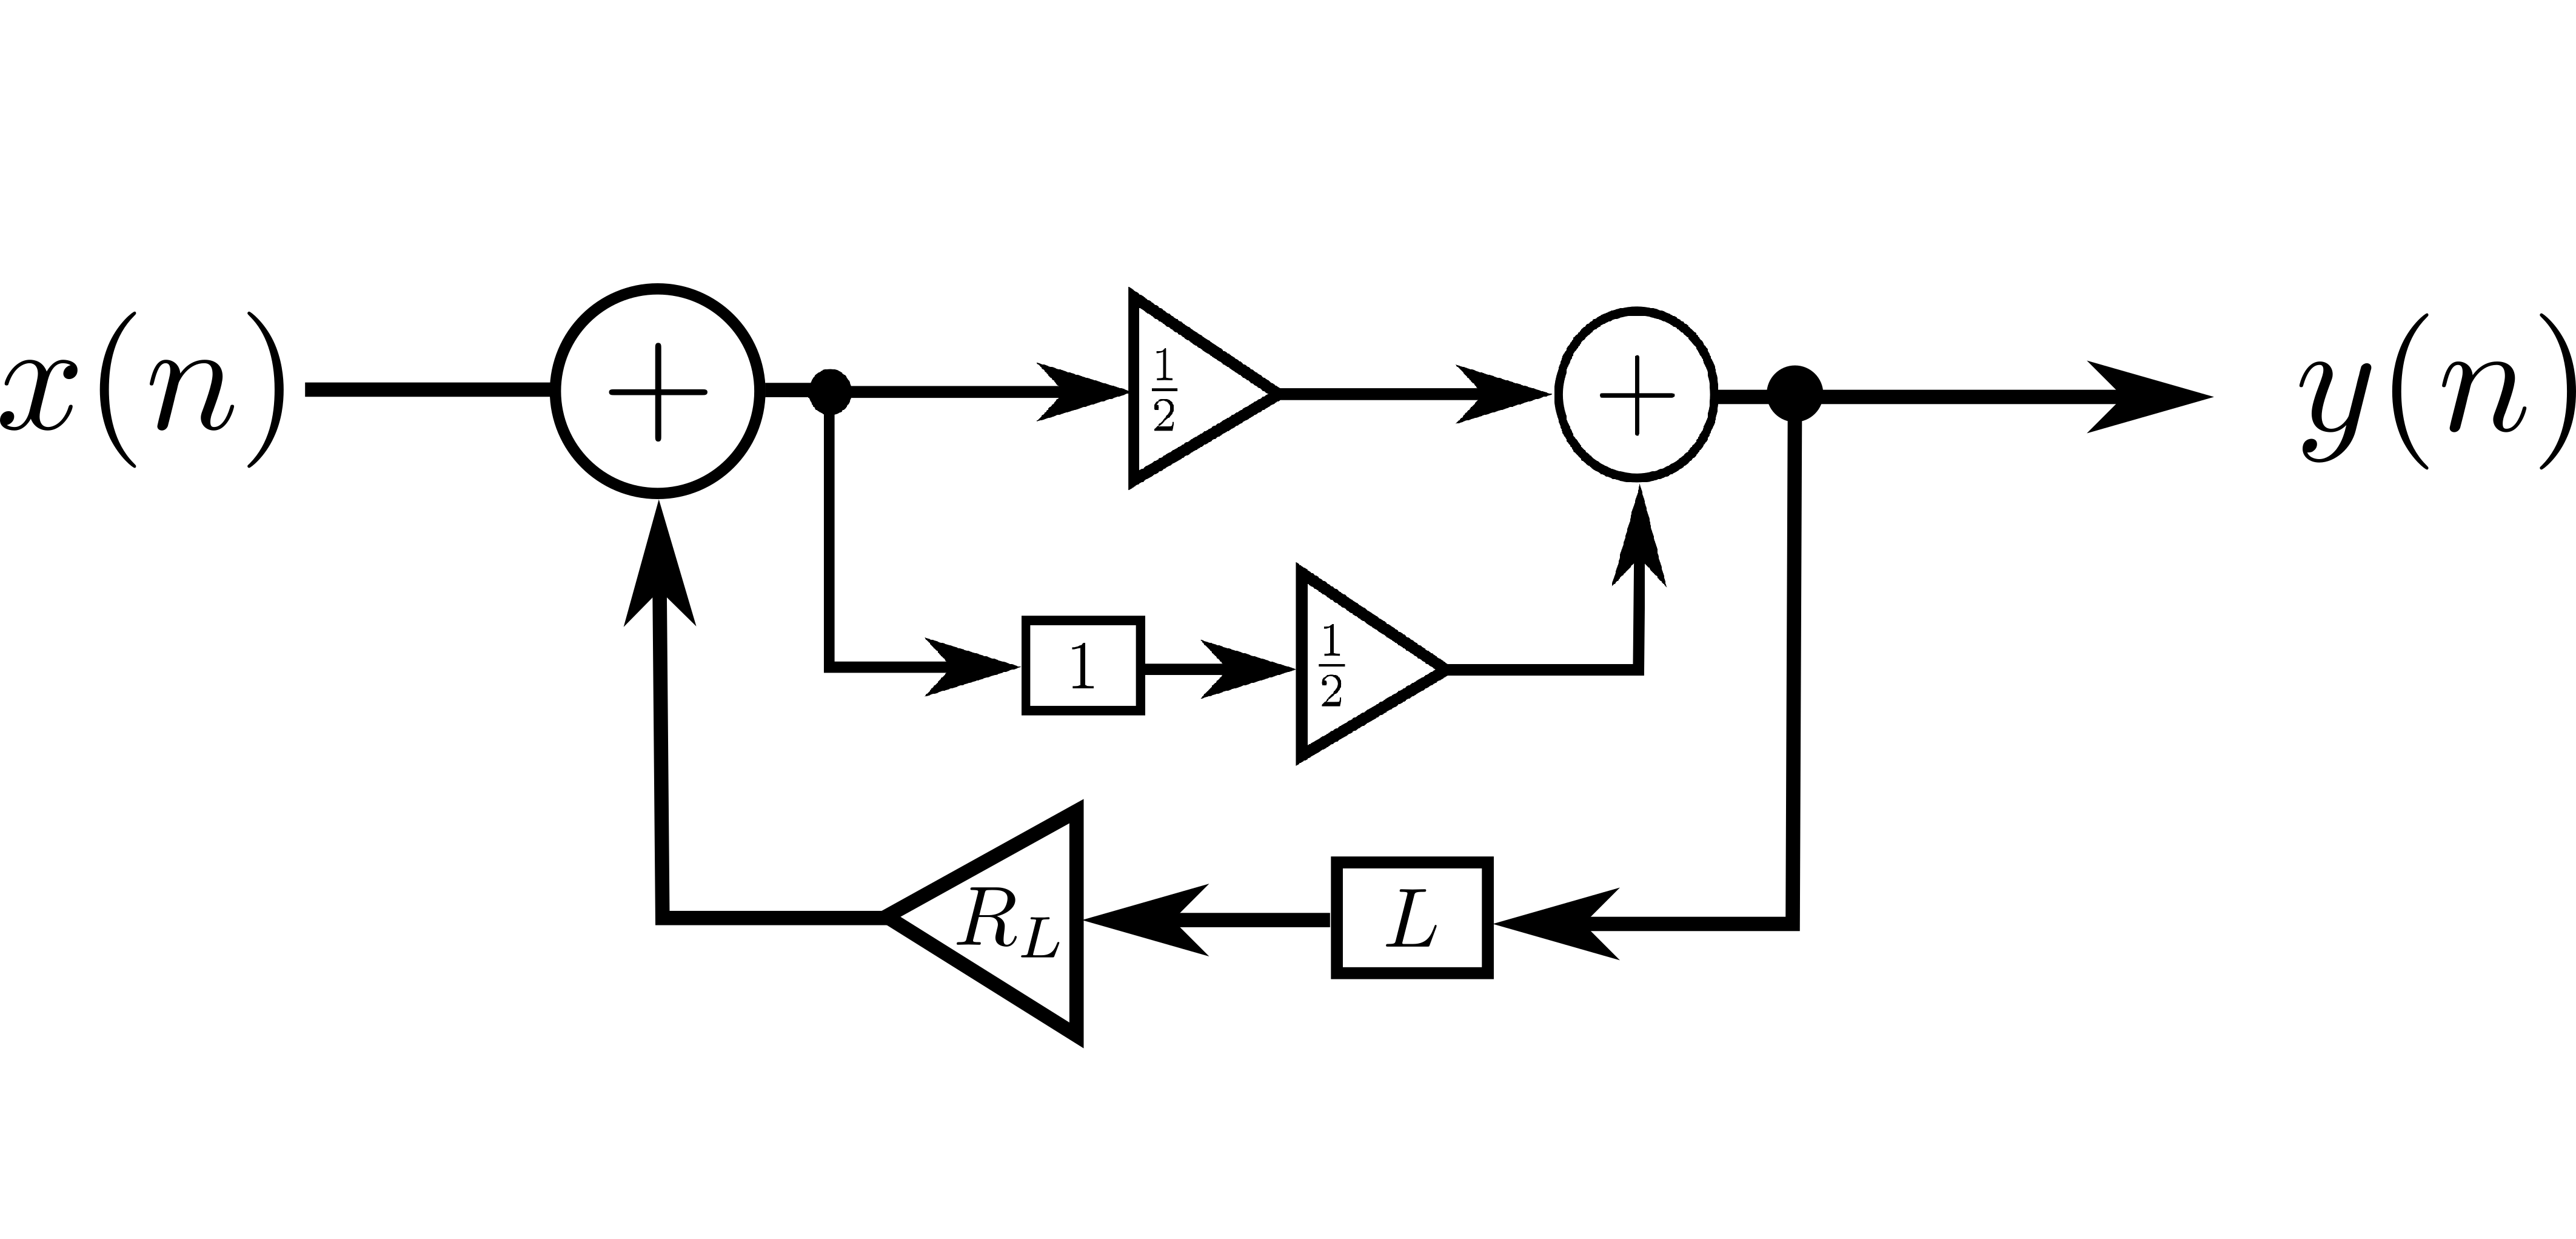
\includegraphics[width=0.8\textwidth]{ImagenesEjercicio4/ksclasic.PNG}
\caption{Algoritmo Karplus-Strong.}
	\label{fig:ksclasico}
\end{figure}
De este diagrama en bloques se puede obtener la ecuación en diferencias:
\begin{align}
y(n) = \frac{1}{2}\cdot x(n) +\frac{1}{2}\cdot x(n-1) + \frac{1}{2}\cdot R_L \cdot y(n-L) + + \frac{1}{2}\cdot R_L \cdot y(n-L-1) 
\label{eq:eqdif}
\end{align}
A partir de esta expresión se puede calcular su transformada Z y depejar para la transferencia:
\begin{align}
H(z) = \frac{\frac{1}{2} \cdot z^{L+1} +\frac{1}{2} \cdot z^{L} }{z^{L+1} - \frac{R_L}{2} \cdot z - \frac{R_L}{2}}
\label{eq:hzks}
\end{align}  
Vale la pena mencionar que de la ecuación (\ref{eq:eqdif}) es una ecuación en diferencias que cuenta como condiciones iniciales la wavetable suministrada por el ruido.
\subsubsection{Análisis singularidades}
Se observa que la expresión (\ref{eq:hzks}) cuenta con L+1 polos y L+1 ceros. A continuación se muestra un diagrama de polos y ceros del sistema:
\begin{figure}[H]
	\centering
	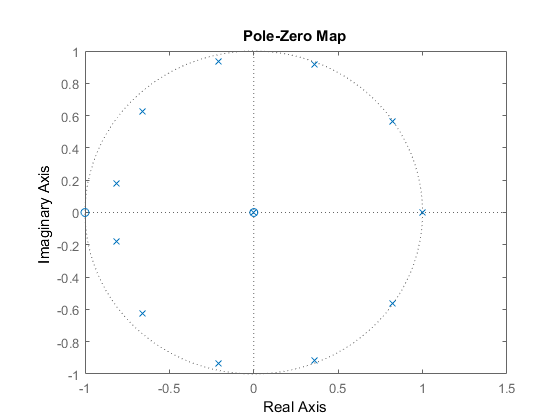
\includegraphics[width=0.8\textwidth]{ImagenesEjercicio4/pzks.PNG}
\caption{Diagrama de polos y ceros.}
	\label{fig:zpdig}
\end{figure}
Adicionalmente se graficó el diagrama de bode del sistema.
\begin{figure}[H]
	\centering
	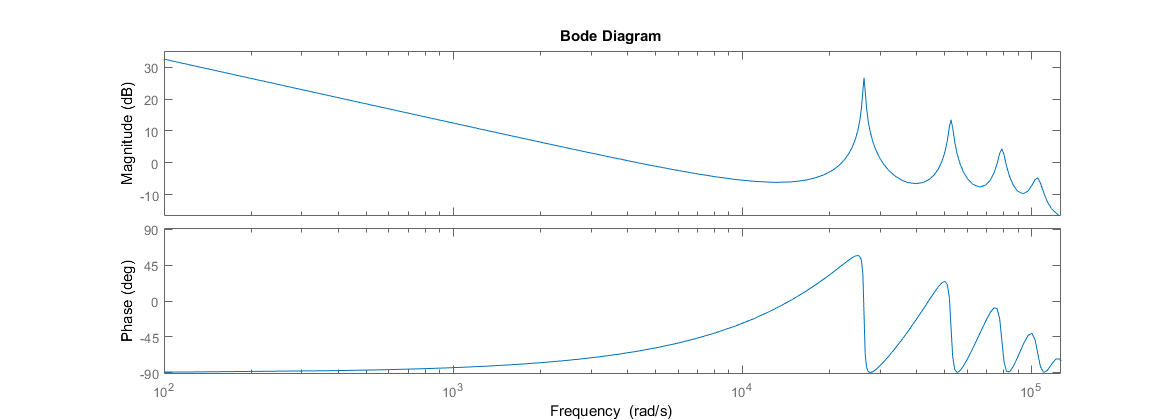
\includegraphics[width=\textwidth]{ImagenesEjercicio4/bodeks.PNG}
\caption{Diagrama de Bode.}
Considerando que los parámetros eran: $f_s = 44.1kHz$, $L=10$ y $R_L=1$
	\label{fig:bode}
\end{figure}

\subsubsection{Sintonización de frecuencia}
En cuanto a la elección de una frecuencia de oscialción se puede observar en los úlitmos gráficos que existe un valor de frecuencia, la cual tiene mayor probabilidad de cumplir el criterio de Barkhausen, la cual corresponde a $f_r = \frac{f_s}{L+0.5}$, esto se debe a que el sistema es la superposición de una linea de retraso  L y otra sistema de retraso L+1, la señal al recorrer el lazo lo hace cada $\frac{L+L+1}{2}$ cambiando esto por frecuencia se obtiene $f_r=\frac{f_s}{L+0.5}$.
\subsubsection{Tipos de ruido}
Se propuso exitar el sistema con distintos tipos de ruido de entrada, siendo estos:
\begin{itemize}
\item Ruido Gaussiano
\item Ruido Uniforme
\item Ruido Binario

\end{itemize}
\subsubsection{Estabilidad}
La estabilidad del sistema será determinada por la ecuación (\ref{eq:hzks}) se puede observar que si RL es mayor o igual a uno el sistema será inestable, si bien teóricamente esto es cierto, en la realidad se encuentra que si RL = 1 no solo no provocará inestablidad, sino que es recomendable este valor dado que logrará extender las oscilaciones  un mayor tiempo.
\subsubsection{Cálculo Fase}
\subsection{Mejora propuesta}
\subsubsection{Análisis teórico}
\subsubsection{Sintonización de frecuencia}
\subsubsection{Continuidad del sonido}
\subsection{Karplus-Strong percución}
\subsection{Espectrogramas}
\end{document}
	
\section{Efectos de Audio}
	\label{Ejercicio-6}
	\documentclass[a4paper]{article}
\usepackage[utf8]{inputenc}
\usepackage[spanish, es-tabla, es-noshorthands]{babel}
\usepackage[table,xcdraw]{xcolor}
\usepackage[a4paper, footnotesep = 1cm, width=20cm, top=2.5cm, height=25cm, textwidth=18cm, textheight=25cm]{geometry}
%\geometry{showframe}

\usepackage{tikz}
\usepackage{amsmath}
\usepackage{amsfonts}
\usepackage{amssymb}
\usepackage{float}
\usepackage{graphicx}
\usepackage{caption}
\usepackage{subcaption}
\usepackage{multicol}
\usepackage{multirow}
\setlength{\doublerulesep}{\arrayrulewidth}
\usepackage{booktabs}
\usepackage{mathrsfs,amsmath}
\usepackage{hyperref}
\hypersetup{
    colorlinks=true,
    linkcolor=blue,
    filecolor=magenta,      
    urlcolor=blue,
    citecolor=blue,    
}

\newcommand{\quotes}[1]{``#1''}
\usepackage{array}
\newcolumntype{C}[1]{>{\centering\let\newline\\\arraybackslash\hspace{0pt}}m{#1}}
\usepackage[american]{circuitikz}
\usetikzlibrary{calc}
\usepackage{fancyhdr}
\usepackage{units} 

\graphicspath{./Imagenes}

\pagestyle{fancy}
\fancyhf{}
\lhead{22.05 ASSD}
\rhead{Mechoulam, Lambertucci, Rodriguez, Londero}
\rfoot{Página \thepage}

\begin{document}
\section{Simulaciones Básicas}

Se simularon las funciones descritas en la Tabla (\ref{fn})

\begin{table}[H]
\centering
\begin{tabular}{@{}c@{}}
\toprule
Función \\ \midrule
$A\cdot Cos(2\pi \cdot 1.5kHz \cdot t)$ \\
Triangular simétrica 1.5kHz de pico $V_{MAX}$ \\
3/2 Seno amplitud VMAX 1.5kHz \\ \bottomrule
\end{tabular}
\caption{Funciones a simular}
\label{fn}
\end{table}

Se determinó que el valor máximo de amplitud de entrada al sistema es de $5V$ el cual es el mínimo entre los dos valores limitantes: Máxima entrada al CD4066 y límite mínimo de distorsión. Además, los límites de tensión de alimentación recomendados son 18V de la hoja de datos del CD4066.

Para hallar los valores óptimos de $A$, $F_s$ y $DT$ se simuló utilizando \textit{LTSpiceXVII} las curvas de entrada y salida del sistema variando simultáneamente los valores de las tres variables, previamente fijando los rangos de variación de las variables. Estos rangos son de $1V$ a $5V$ para $A$,
 $21kHz$ (para cumplir con el doble de la frecuencia de corte del filtro recuperador) a $25kHz$ (límite del oscilador) y de $5\%$ (límite del oscilador) a $50\%$ (limite por consigna) para el duty cycle. Finalmente, se utilizó el siguiente script en \textit{Python} para hallar el valor de las tres variables tal que la distorsión a la salida respecto a la entrada sea la mínima, computando la correlación entre las dos señales.

\lstinputlisting{Python/spiceanal.py}

Esto dio los siguientes resultados:

\begin{figure}[H]
\centering
\begin{subfigure}{\linewidth}
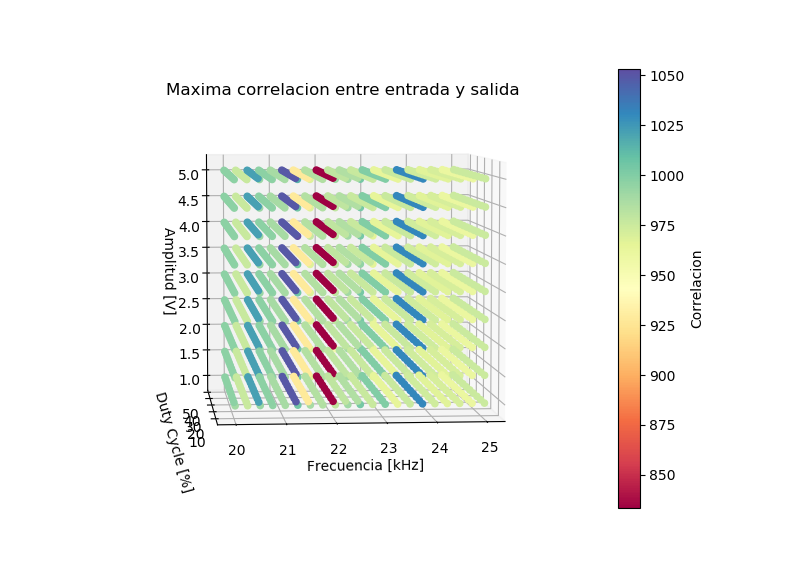
\includegraphics[width=\linewidth]{ImagenesEjercicio6/scatter_sh_seno.png}
\caption{Scatterplot de las simulación.}
\end{subfigure}

\begin{subfigure}{\linewidth}
\[A = 4V \ F_s = 21250Hz \ DT = 5\%\]
\caption{Parámetros para la menor distorsión.}
\end{subfigure}
\label{seno_sh}
\caption{Resultados experimentales de la simulación para \textbf{senoidal con S\&H}.}
\end{figure}

\begin{figure}[H]
\centering
\begin{subfigure}{\linewidth}
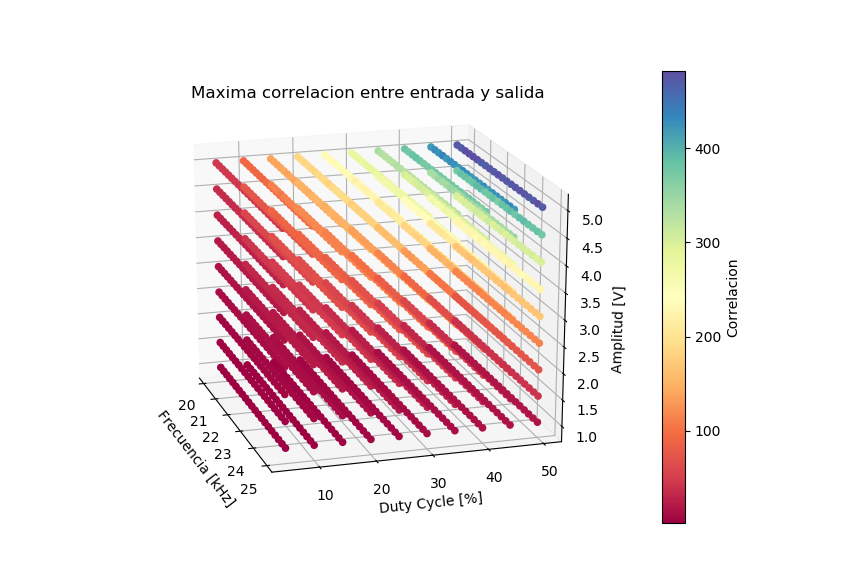
\includegraphics[width=\linewidth]{ImagenesEjercicio6/scatter_llave_seno.png}
\caption{Scatterplot de las simulación.}
\end{subfigure}

\begin{subfigure}{\linewidth}
\[A = 5V \ F_s = 21250Hz \ DT = 50\%\]
\caption{Parámetros para la menor distorsión.}
\end{subfigure}
\label{seno_llave}
\caption{Resultados experimentales de la simulación para \textbf{senoidal con llave analógica}.}
\end{figure}

\begin{figure}[H]
\centering
\begin{subfigure}{\linewidth}
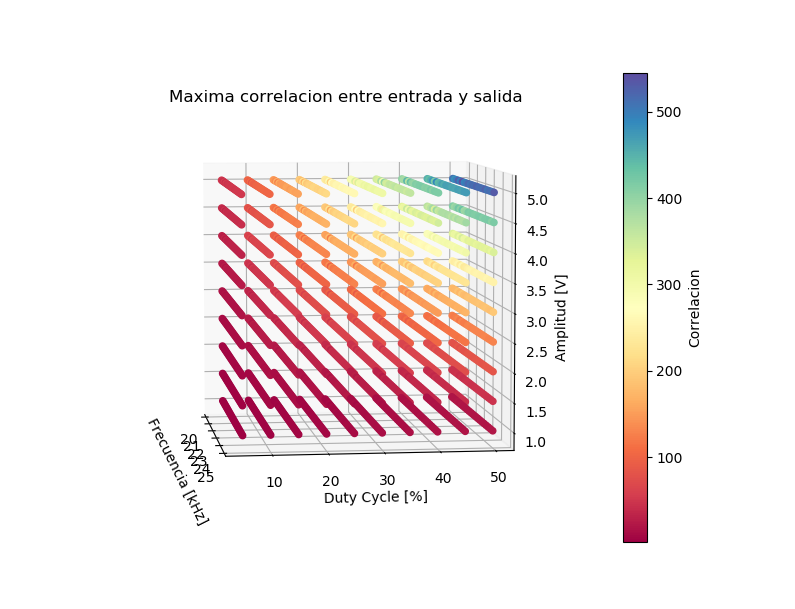
\includegraphics[width=\linewidth]{ImagenesEjercicio6/scatter_llave_triang.png}
\caption{Scatterplot de las simulación.}
\end{subfigure}

\begin{subfigure}{\linewidth}
\[A = 5V \ F_s = 23750Hz \ DT = 50\%\]
\caption{Parámetros para la menor distorsión.}
\end{subfigure}
\label{triang_llave}
\caption{Resultados experimentales de la simulación para \textbf{triangular con llave analógica}.}
\end{figure}

\begin{figure}[H]
\centering
\begin{subfigure}{\linewidth}
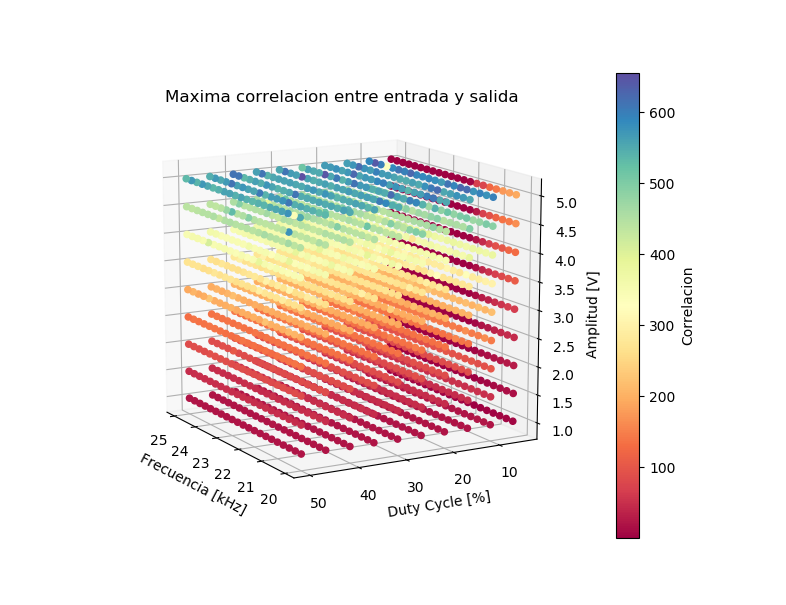
\includegraphics[width=\linewidth]{ImagenesEjercicio6/scatter_sh_triang.png}
\caption{Scatterplot de las simulación.}
\end{subfigure}

\begin{subfigure}{\linewidth}
\[A = 5V \ F_s = 24000Hz \ DT = 30\%\]
\caption{Parámetros para la menor distorsión.}
\end{subfigure}
\label{triang_sh}
\caption{Resultados experimentales de la simulación para \textbf{triangular con S\&H}.}
\end{figure}

\begin{figure}[H]
\centering
\begin{subfigure}{\linewidth}
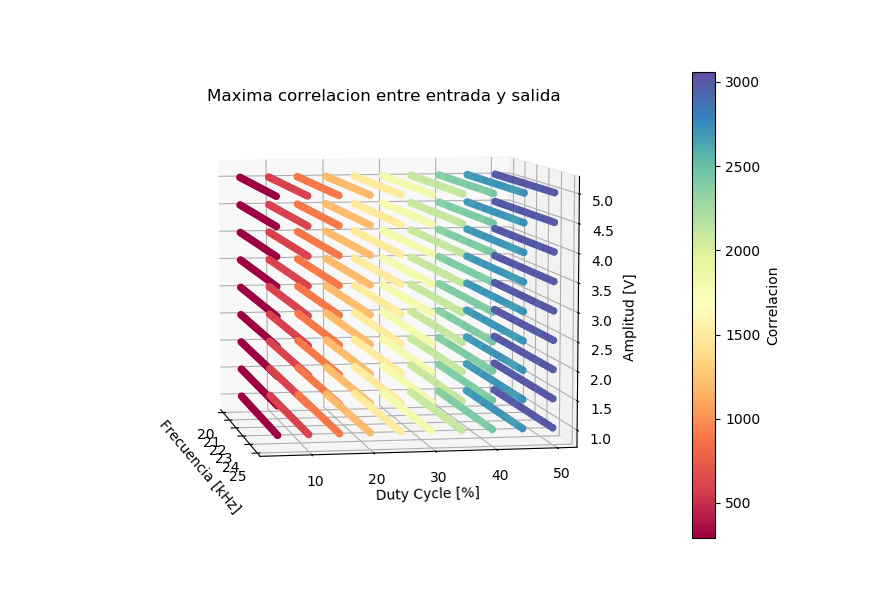
\includegraphics[width=\linewidth]{ImagenesEjercicio6/scatter_llave_sen32.png}
\caption{Scatterplot de las simulación.}
\end{subfigure}

\begin{subfigure}{\linewidth}
\[A = 1V \ F_s = 23500Hz \ DT = 50\%\]
\caption{Parámetros para la menor distorsión.}
\end{subfigure}
\label{sen32_llave}
\caption{Resultados experimentales de la simulación para \textbf{seno 3/2 con llave analógica}.}
\end{figure}

\begin{figure}[H]
\centering
\begin{subfigure}{\linewidth}
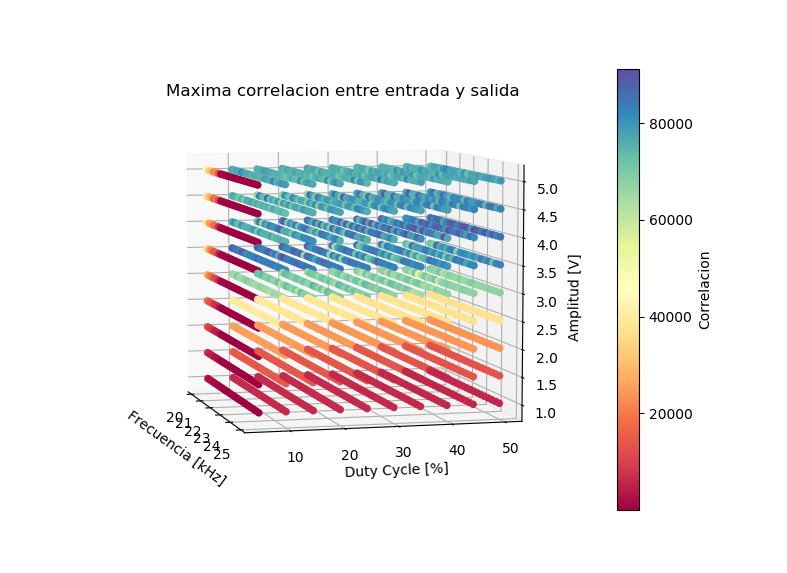
\includegraphics[width=\linewidth]{ImagenesEjercicio6/scatter_sh_sen32.png}
\caption{Scatterplot de las simulación.}
\end{subfigure}

\begin{subfigure}{\linewidth}
\[A = 1.5V \ F_s = 20000Hz \ DT = 5\%\]
\caption{Parámetros para la menor distorsión.}
\end{subfigure}
\label{sen32_sh}
\caption{Resultados experimentales de la simulación para \textbf{seno 3/2 con S\&H}.}
\end{figure}

\subsubsection{Simulaciones con Python}
Se utilizó el framework de \textbf{GNURadio} para programar cada módulo del sistema encerrado en una interfaz gráfica, la cual brinda la posibilidad de visualizar tanto la señal en tiempo como su espectro en cada nodo del sistema en el mismo momento. Se puede elegir entre señales sinusoidales, triangulares, 3/2 seno o moduladas AM como entrada, señales cuyo estudio es de interes.

\subsubsection{Simulaciones con LTSpice}
Para ambos sistemas, tanto con la llave analógica seleccionada como para el Sample and Hold elegido, se realizaron las simulaciones de las funciones en la Tabla (\ref{fn}) con las exitaciones deseadas con los siguientes esquemas en \textit{LTSPICEXVII}.

\begin{figure}[H]
\centering
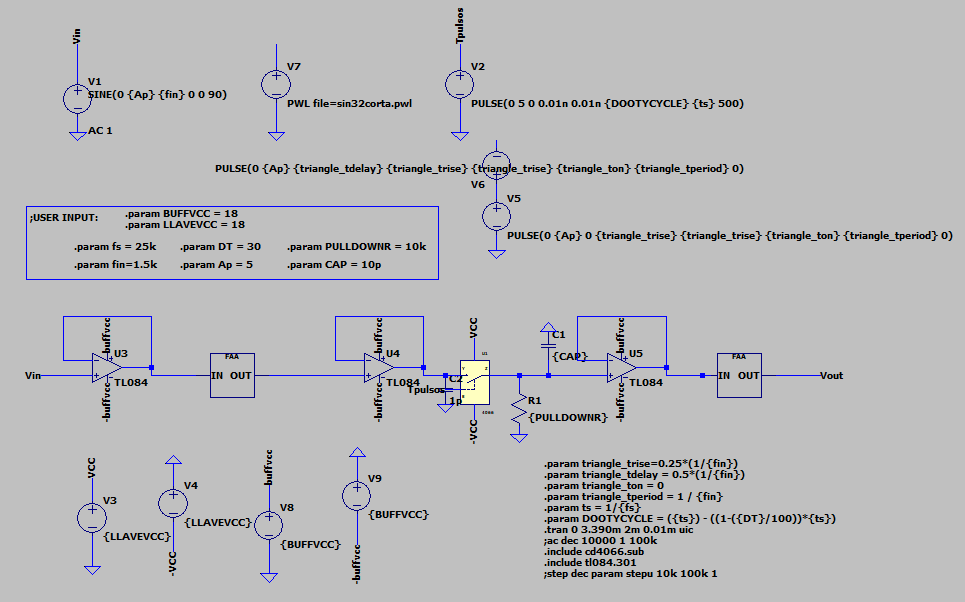
\includegraphics[width=\textwidth]{ImagenesEjercicio6/SIMULACIONLLAVE.png}
\caption{Esquema de simulación para el sistema con llave analógica.}
\end{figure}

\begin{figure}[H]
\centering
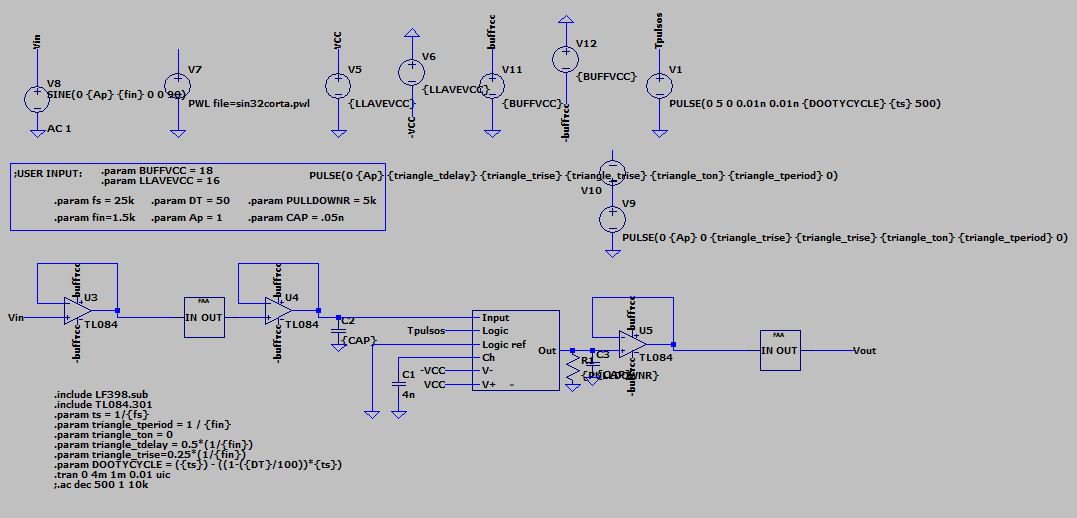
\includegraphics[width=\textwidth]{ImagenesEjercicio6/SIMULACIONSH.png}
\caption{Esquema de simulación para el sistema con Sample and Hold.}
\end{figure}

\textcolor{red}{\textbf{Calcular potencia recuperada.}}

Nuevamente, se realizaron las mismas simulaciones variando...

\textcolor{red}{\textbf{Aclarar bajo qué condiciones, es el punto 6b.}}

\end{document}


\section{Programas implementados}
	\label{Ejercicio-8}
	\documentclass[a4paper]{article}
\usepackage[utf8]{inputenc}
\usepackage[spanish, es-tabla, es-noshorthands]{babel}
\usepackage[table,xcdraw]{xcolor}
\usepackage[a4paper, footnotesep = 1cm, width=20cm, top=2.5cm, height=25cm, textwidth=18cm, textheight=25cm]{geometry}
%\geometry{showframe}

\usepackage{tikz}
\usepackage{amsmath}
\usepackage{amsfonts}
\usepackage{amssymb}
\usepackage{float}
\usepackage{graphicx}
\usepackage{caption}
\usepackage{subcaption}
\usepackage{multicol}
\usepackage{multirow}
\setlength{\doublerulesep}{\arrayrulewidth}
\usepackage{booktabs}
\usepackage{mathrsfs,amsmath}
\usepackage{hyperref}
\hypersetup{
    colorlinks=true,
    linkcolor=blue,
    filecolor=magenta,      
    urlcolor=blue,
    citecolor=blue,    
}

\newcommand{\quotes}[1]{``#1''}
\usepackage{array}
\newcolumntype{C}[1]{>{\centering\let\newline\\\arraybackslash\hspace{0pt}}m{#1}}
\usepackage[american]{circuitikz}
\usetikzlibrary{calc}
\usepackage{fancyhdr}
\usepackage{units} 

\graphicspath{./Imagenes}

\pagestyle{fancy}
\fancyhf{}
\lhead{22.05 ASSD}
\rhead{Mechoulam, Lambertucci, Rodriguez, Londero}
\rfoot{Página \thepage}

\begin{document}
\subsection{FFT}
Se implementó la FFT utilizando el algoritmo de Cooley-Tukey de manera recursiva.
Se probó con diversas entradas reales aleatorias, de tamaño 4096, con una media temporal de 40$\mu$s.
\subsection{Programa Principal}
La GUI implementada es la siguiente:
\begin{figure}[H]
	\centering
	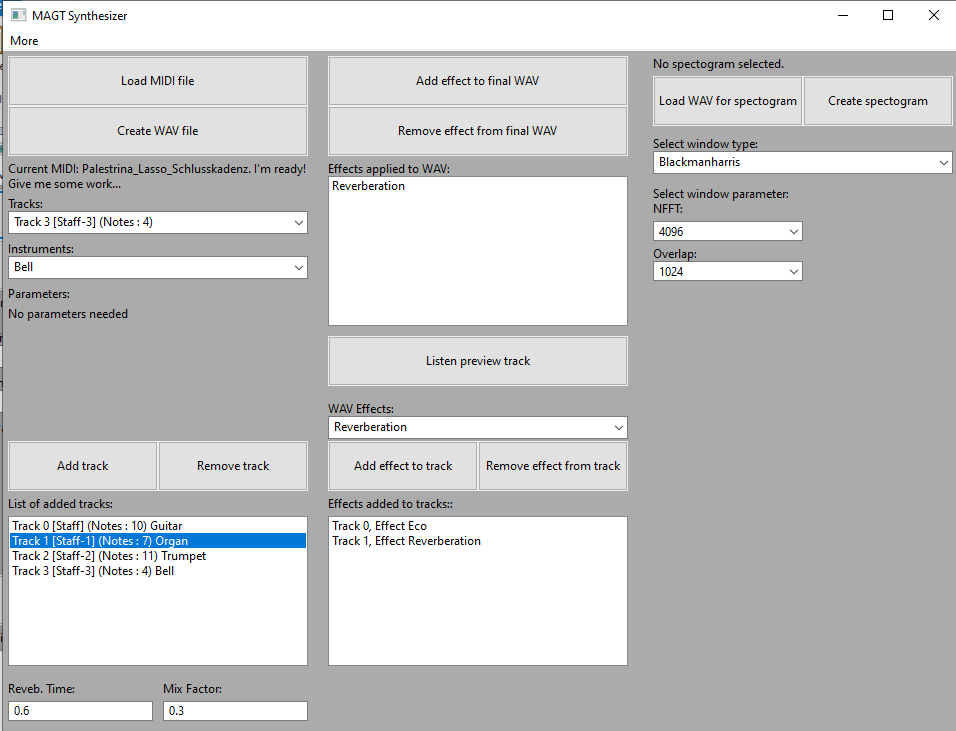
\includegraphics[width=0.8\textwidth]{ImagenesEjercicio8/GUI.PNG}
\caption{GUI Implementada.}
	\label{fig:gui}
\end{figure}
Permite agregar midis de cualquier duración, sintetizar cada track con el instrumento deseado, al igual que escuchar un preview del mismo, funcionalidad de pantalla completa, una sección de ayuda al usuari; Ademas permite la mezcla tracks, agregar efectos tanto a los tracks como al proyecto entero. Realizar espectrogramas de los wavs generados, pudiendo elegir el tipo de ventana, la cantidad de puntos de la FFT y el overlap. Ademas permite manejar los parametros de algunos instrumentos y efectos.\\
El front-end del programa se implemento en WxWidgets. El programa fue desarrollado en C++. \\

\end{document}


\end{document}